\subsection{Bluetooth}
\label{subsection:bt}

A \gls{WPAN} is type of network where devices are connected wirelessly to each other, based on the standard IEEE 802.15. This definition seems to be quite similar to the one of \gls{WLAN}, but there is a considerable number of differences between the two. The term personal area network derives from the use that is to be given to such networks, in other words, \glspl{WPAN} are to be deployed in order to connect multiple devices of one's personal area, such as home, office, \textit{etc.}.

Bluetooth is one of the main technologies to implement a \gls{WPAN}, described above. It uses the 2.4GHz \gls{ISM} band, it was invented by phone company Ericsson, and is used to connect devices in a short range network.

Devices connect to each other forming \textit{piconets}, which is the term assigned to designate an ad hoc network formed by devices using Bluetooth. Each \textit{piconet} has a master, the device that controls the network, similarly to an \gls{AP} without providing access to the infrastructured network. Associated to each master there can be up to seven slaves, which are devices that take part in the same \textit{piconet}. Multiple \textit{piconets} can connect between themselves and form a \textit{scatternet}, as seen in figure \ref{fig:bluetooth}:

\begin{figure}[ht]
	\noindent\makebox[\textwidth]
    {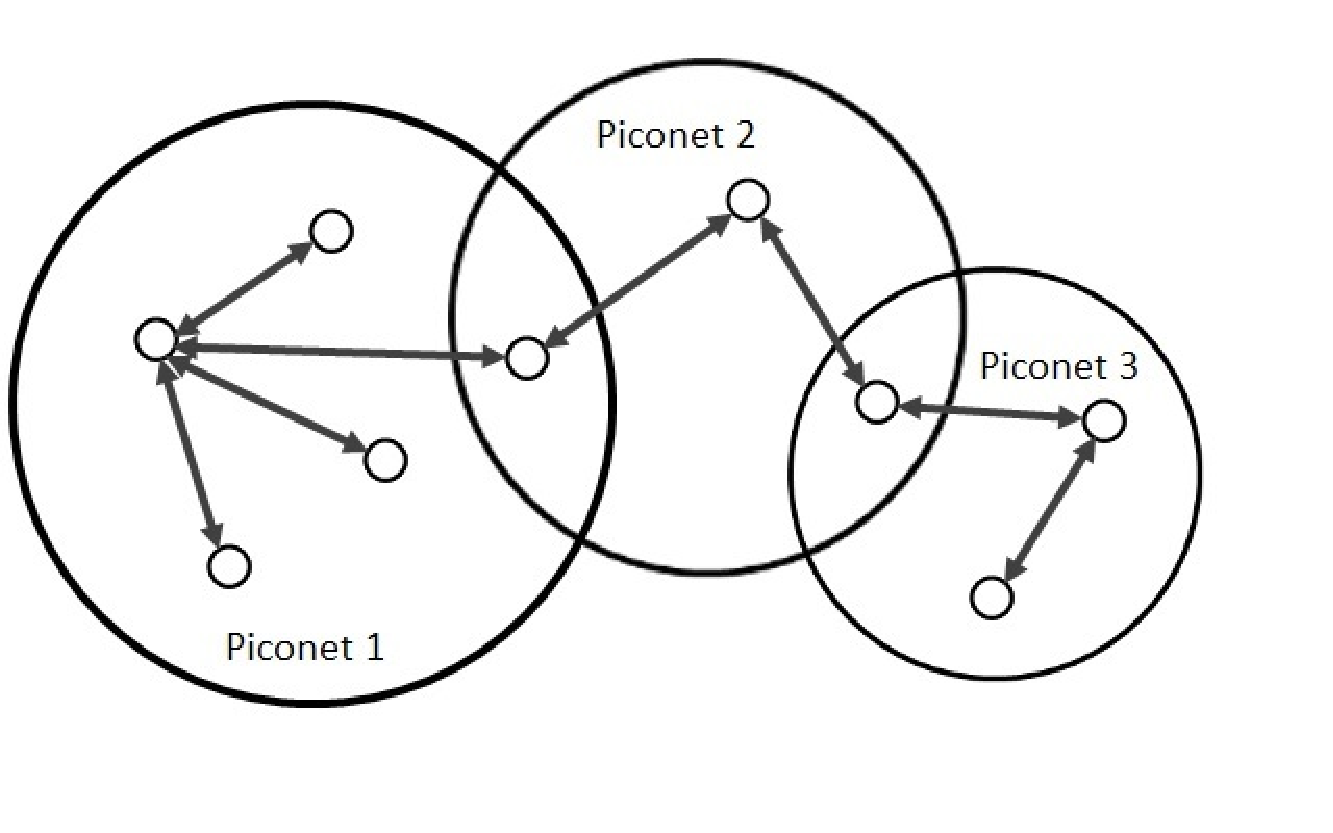
\includegraphics[scale=0.5]{images/bluetooth.pdf}}
	\caption{\label{fig:bluetooth} Scatternet Layout (adapted from: www.summitdata.com)}
\end{figure}

Each master is associated with a certain number of slaves, that can participate in more than one piconet, as seen above. These slaves are responsible for coordinating both \textit{piconets}, so that no interference exists.

Bluetooth uses slow \gls{FHSS} to control the frequency of transmission of each slave, this is done by creating a hopping sequence partially based on the master device's \gls{MAC} address, and then distributing the sequence to each slave on the \textit{piconet}. Devices connect to the \textit{piconet} by pairing with the master, forming a secure link, the master then controls the access to the medium by deciding which slave will transmit at a certain moment in time. In the \textit{scatternet} case, the data to be transmitted from \textit{piconet} to \textit{piconet} is relayed by the node participating in both networks. The pairing of both \textit{piconets} is similar to the pairing of a master and a new member of the network.

Although several advantages of Bluetooth are clear, such as low power wireless protocol, low transmission headers, ease of set up, multi group information transfer, this protocol still has a lot of downsides. The main current problems with Bluetooth consist in the low range of connections, due to the week signal power being a feature of the technology, the limited number of users that can form a \textit{piconet}, due to the narrow band used by Bluetooth and, finally, the low data rates of the protocol, which are heavily surpassed by the Wi-Fi standard.

\gls{WPAN} uses, typically, technologies that allow communication between devices within a certain specific range, usually around 10 meters, making this type of network much smaller than the ones created by \gls{WLAN}. The most common technology is Bluetooth, although there are several other technologies that are beginning to raise awareness, due to the crescent interest taken in \gls{IoT}, such as ZigBee. The used radio band is the 2.4 GHz \gls{ISM} band, due to its general availability worldwide and its lower cost.

\gls{BLE} is the power-version of Bluetooth developed for \gls{IoT}. The natural power-efficiency of Bluetooth combined with lower energy consumption provides the key factors for devices running for long periods of time without recharging. \gls{BLE}'s key features include: standard wireless protocol, allowing for interoperability across platforms, low idle power consumption and data encryption for security of communications, among others.

\gls{BLE} achieves data rates similar to classic Bluetooth over the same distance, although the application throughputs are much smaller: 0.27Mbps compared to 0.7-2.1Mbps for classic Bluetooth. The spectrum range of \gls{BLE} is the same as in classic Bluetooth, but the channels are two times wider than in Classic, consequently, there is half the number of channels. The main difference between the two lies in the power consumption and peak current consumption, 0.01-0.5W and less than 15mA for \gls{BLE}, 1W and less than 30mA for classic Bluetooth. The number of slaves in \gls{BLE} is implementation dependent as opposed to the fixed seven in classic Bluetooth.

\gls{BLE} is appropriate for networks that rely on the longevity of the battery of the devices, application throughputs are smaller but the information to be sent is, usually, also much less than in classic Bluetooth. One of the biggest limitation of \gls{BLE} is the inability to transmit voice, whereas classic Bluetooth is able. Despite this and other disadvantages of \gls{BLE} there are many areas that can benefit from technologies such as this one, \textit{e.g.} healthcare applications, logistic sensors, sports, among others, so it is not a technology that should be overlooked.











